% Saberes básicos (LOMLOE) asociados a esta unidad
%
% Bloque A. Las destrezas científicas básicas
%   - Uso del lenguaje científico y de las unidades del Sistema Internacional (SI):
%     la unidad se trabaja con el julio y sus múltiplos/submúltiplos, además de otras
%     unidades de energía de uso habitual (caloría, kWh, tep), reforzando el manejo
%     correcto de magnitudes y unidades ya introducido en la Unidad 1.
%
% Bloque C. La energía
%   - Formulación de cuestiones e hipótesis sobre la energía, sus propiedades y
%     manifestaciones como causa de todos los procesos de cambio: se define la energía,
%     sus formas (cinética, potencial, térmica, eléctrica, radiante, química, nuclear)
%     y sus propiedades (se transfiere, se almacena, se transporta, se transforma,
%     se degrada y se conserva).
%   - Diseño y comprobación experimental de hipótesis sobre el uso doméstico e industrial
%     de la energía y las transformaciones entre sus distintas formas: se analizan cadenas
%     de transformación energética en aparatos cotidianos (linterna, secador, aerogenerador,
%     hervidor, panel solar) y el concepto de degradación/rendimiento.
%   - Elaboración fundamentada de hipótesis sobre el medio ambiente y la sostenibilidad a
%     partir de las diferencias entre fuentes renovables y no renovables. Valoración de la
%     producción de energía eólica en Castilla-La Mancha: se dedica un apartado específico
%     a la energía eólica en la región, con sus ventajas y sus impactos.
%   - Efectos del calor sobre la materia: se incorpora un apartado sobre el calor específico
%     y la dilatación térmica, con ejemplos y aplicaciones cotidianas (juntas de dilatación,
%     termómetros de líquido, clima costero frente a clima de interior).
%   - Naturaleza eléctrica de la materia: electrización de los cuerpos, circuitos eléctricos
%     y obtención de energía eléctrica: se desarrollan la ley de Ohm y los circuitos en serie
%     y en paralelo, junto con el ahorro energético y la conservación sostenible del medio
%     ambiente, ya tratados en la unidad.

\spacing{1.3}
\raggedbottom % pages with large figures end where the text ends (no stretched gaps between boxes)

\section{What is energy?}

\begin{definition}[Energy]
    A physical quantity that measures the capacity of a body to produce changes in itself or in other bodies.
\end{definition}

Whenever a person, a machine or any other object does something, it uses energy and has to get more in order to keep working.

\begin{didyouknow}
    Your brain uses about 20\,\% of all the energy your body gets from food, even though it is only about 2\,\% of your body mass!
\end{didyouknow}

\subsection{How is energy measured?}

In the SI, energy is measured in \textbf{joules} (J); the kilojoule (\qty{1}{\kj} = \qty{1000}{\joule}) is also common. There are also other units, used in specific fields:

\begin{itemize}
    \item \negsubro{Calorie} (cal): the amount of heat needed to raise the temperature of \qty{1}{\g} of water by \qty{1}{\celsius}. \(\qty{1}{\calorie} = \qty{4.18}{\joule}\). Food energy is traditionally given in Calories (with a capital C): \(1 \text{ Calorie} = 1000 \text{ calories} = \qty{1}{\kilo\calorie}\).
    \item \negsubro{Kilowatt-hour} (kWh): used to measure electrical energy; it is the energy consumed by a \qty{1}{\kW} appliance used for one hour. \(\qty{1}{\kwh} = \qty{3.6e6}{\joule}\).
    \item \negsubro{Tonne of oil equivalent} (toe): used in the oil industry; it is the energy obtained by burning \qty{1000}{\kg} of petroleum. \(1 \text{ toe} \approx \qty{4.187e10}{\joule}\).
\end{itemize}

\begin{figure}[H]
    \centering
    % [FIGURA ORIGINAL] \includegraphics[width=\textwidth]{Unit_9/energy_units}
    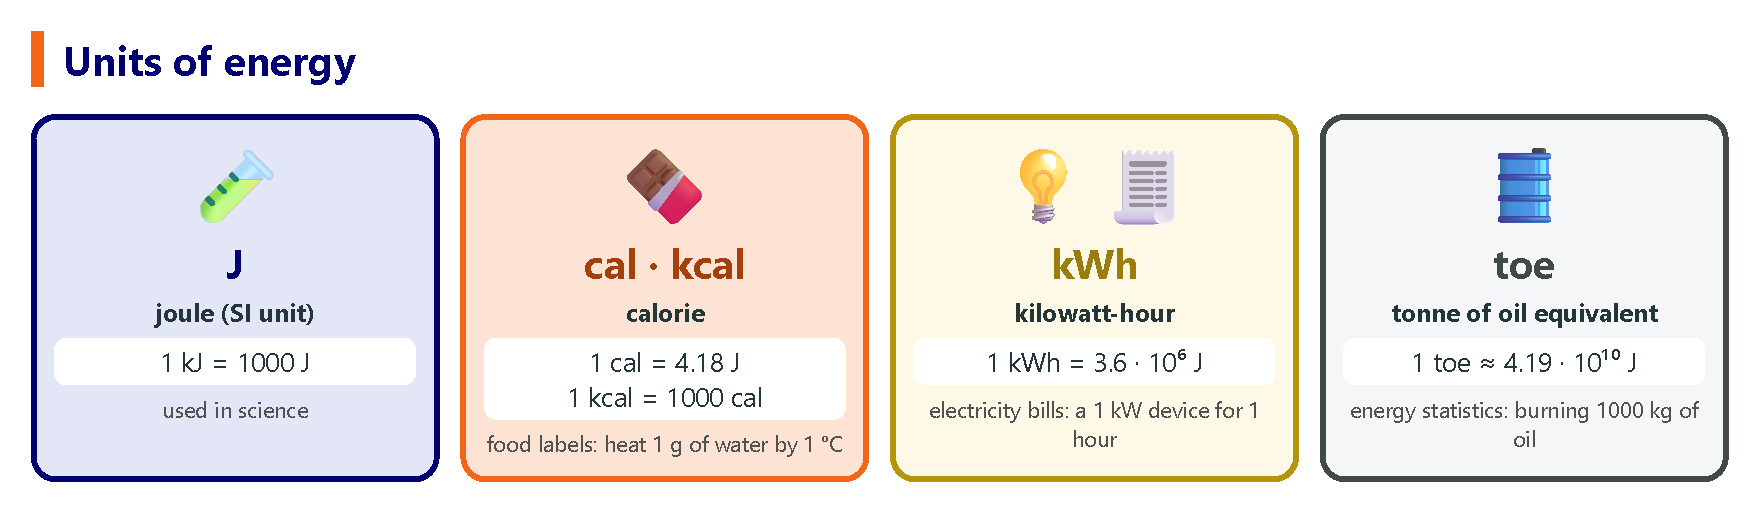
\includegraphics[width=\textwidth]{FigurasSVG/Unit_9_Energy/pdf/energy_units.pdf}
    \caption{The most common units of energy and where we find them.}
    \label{fig:u9_energy_units}
\end{figure}

\begin{example}
    \textbf{A ball falls from a basket to the floor with an energy of \qty{18.2}{\joule}. Write this amount in kJ, cal and kWh.}
    \begin{align*}
        \qty{18.2}{\joule} \cdot \dfrac{\qty{1}{\kilo\joule}}{\qty{1000}{\joule}} &= \textbf{0.018 kJ} \\
        \qty{18.2}{\joule} \cdot \dfrac{\qty{1}{\calorie}}{\qty{4.18}{\joule}} &= \textbf{4.35 cal} \\
        \qty{18.2}{\joule} \cdot \dfrac{\qty{1}{\kwh}}{\qty{3.6e6}{\joule}} &\approx \textbf{5.06} \times \textbf{10}^{\textbf{-6}} \textbf{ kWh}
    \end{align*}
\end{example}

\begin{exercise}
    To make a cup of tea, water is heated from \qty{20}{\celsius} to \qty{100}{\celsius} in a microwave that supplies \qty{83860}{\joule}.
    \begin{enumerate}[label=\letraminuscula]
        \item How many calories is this?
        \item How many kWh is it?
    \end{enumerate}
    \begin{solu}
        \begin{enumerate}[label=\alph*)]
            \item \(\qty{83860}{\joule} \cdot \dfrac{\qty{1}{\calorie}}{\qty{4.18}{\joule}} \approx 20062\) cal.
            \item \(\qty{83860}{\joule} \cdot \dfrac{\qty{1}{\kwh}}{\qty{3.6e6}{\joule}} \approx 0.0233\) kWh.
        \end{enumerate}
    \end{solu}
\end{exercise}

\begin{exercise}
    The energy content of \qty{100}{\g} of biscuits is approximately \qty{350}{\kilo\calorie}. Write this amount in joules.
    \begin{solu}
        \(\qty{350}{\kilo\calorie} = \qty{350000}{\calorie}\); \(\qty{350000}{\calorie} \cdot \qty{4.18}{\joule\per\calorie} \approx \qty{1463000}{\joule} \approx \qty{1.46}{\mega\joule}\).
    \end{solu}
\end{exercise}

\begin{exercise}
    A washing machine uses \qty{1.1}{\kwh} of electrical energy to complete a wash cycle.
    \begin{enumerate}[label=\letraminuscula]
        \item Convert this energy into joules.
        \item Convert this energy into calories.
    \end{enumerate}
    \begin{solu}
        \begin{enumerate}[label=\alph*)]
            \item \(\qty{1.1}{\kwh} \cdot \qty{3.6e6}{\joule\per\kwh} = \qty{3960000}{\joule} \approx \qty{3.96}{\mega\joule}\).
            \item \(\qty{3960000}{\joule} \cdot \dfrac{\qty{1}{\calorie}}{\qty{4.18}{\joule}} \approx 947368\) cal \(\approx 947.4\) kcal.
        \end{enumerate}
    \end{solu}
\end{exercise}

\begin{exercise}
    A solar panel installation produces \qty{2.5}{\mega\joule} of energy in a day. Express this amount in kWh and in kcal.
    \begin{solu}
        \(\qty{2.5}{\mega\joule} = \qty{2500000}{\joule}\). \\
        In kWh: \(\qty{2500000}{\joule} \cdot \dfrac{\qty{1}{\kwh}}{\qty{3.6e6}{\joule}} \approx \textbf{0.694 kWh}\). \\
        In kcal: \(\qty{2500000}{\joule} \cdot \dfrac{\qty{1}{\calorie}}{\qty{4.18}{\joule}} \approx 598086\) cal \(\approx \textbf{598.1 kcal}\).
    \end{solu}
\end{exercise}

%----------------------------------------------------------------------------------------

\section{Forms of energy}

\begin{figure}[H]
    \centering
    % [FIGURA ORIGINAL] \includegraphics[width=\textwidth]{Unit_9/forms_energy}
    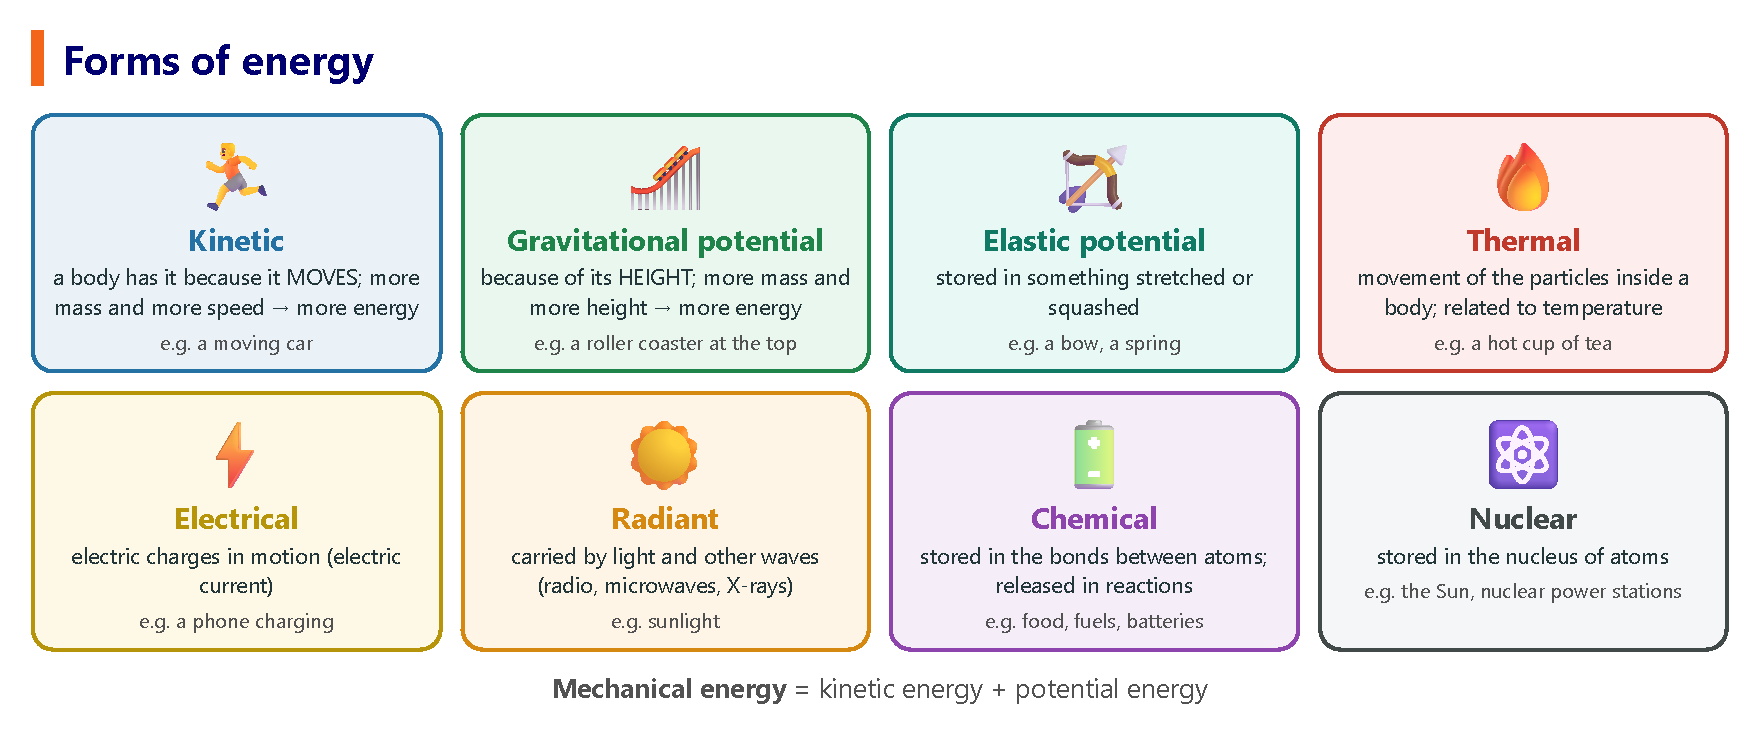
\includegraphics[width=\textwidth]{FigurasSVG/Unit_9_Energy/pdf/forms_energy.pdf}
    \caption{The forms of energy.}
    \label{fig:u9_forms_energy}
\end{figure}

\begin{impt}
    \negsubro{Nuclear fusion vs.\ nuclear fission}:
    \begin{itemize}
        \item \textbf{Nuclear fusion}: light atoms join together to form larger atoms, releasing energy (this happens in the Sun and other stars).
        \item \textbf{Nuclear fission}: heavy atoms break apart into smaller atoms, releasing energy (this happens in nuclear power stations).
    \end{itemize}
\end{impt}

\begin{figure}[H]
    \centering
    % [FIGURA ORIGINAL] \includegraphics[width=\textwidth]{Unit_9/fusion_fission}
    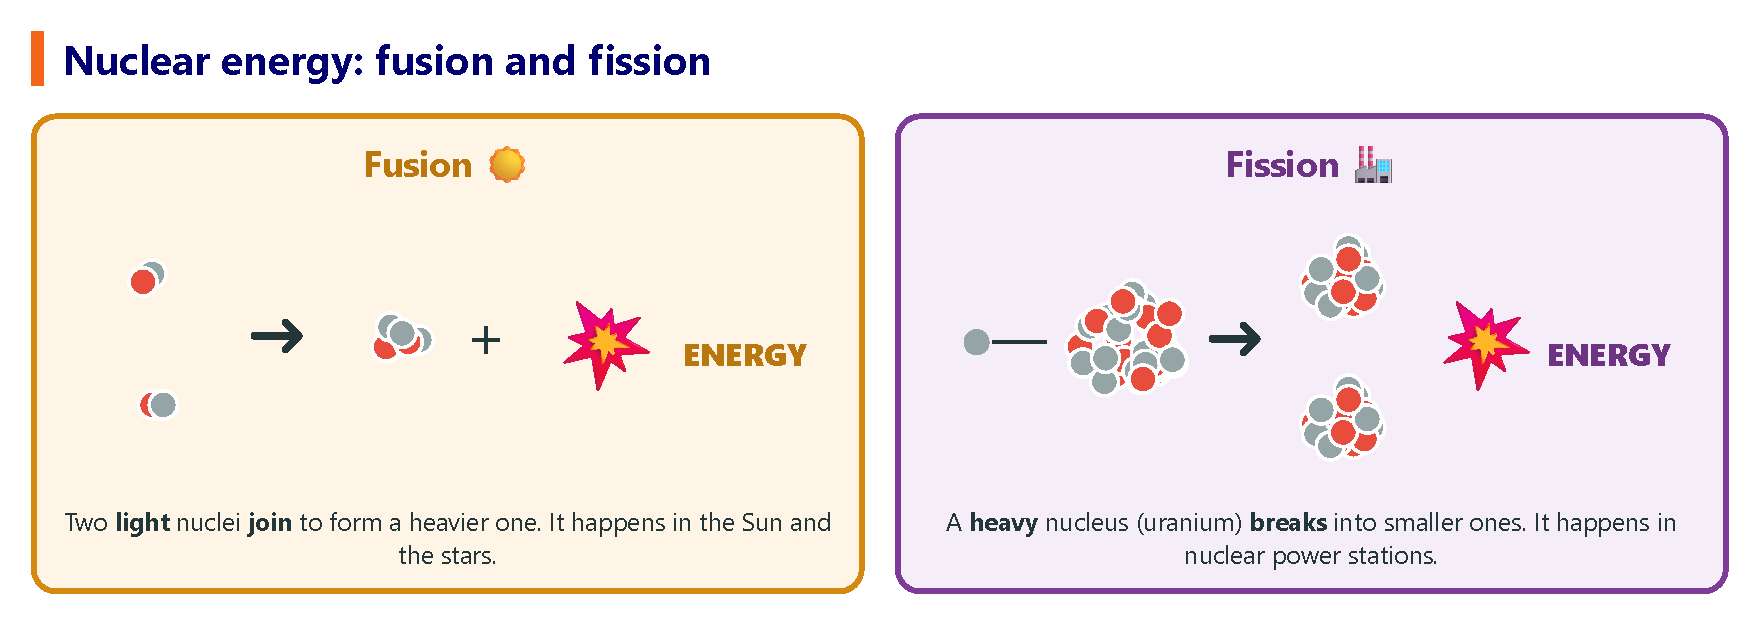
\includegraphics[width=\textwidth]{FigurasSVG/Unit_9_Energy/pdf/fusion_fission.pdf}
    \caption{Nuclear fusion and nuclear fission.}
    \label{fig:u9_fusion_fission}
\end{figure}

\begin{didyouknow}
    Every second, the Sun turns about 4 million tonnes of matter into energy by nuclear fusion. It has been doing this for 4\,600 million years, and it still has fuel for about 5\,000 million years more!
\end{didyouknow}

\begin{example}
    A lorry and a car travel at the same speed; the lorry has more \textbf{kinetic energy} because it has more mass. The same car has more kinetic energy when it travels faster. A ball has more \textbf{gravitational potential energy} the higher it is and the more mass it has. A stretched bow has more \textbf{elastic potential energy} the more it is stretched.
\end{example}

\begin{exercise}
    Say which form(s) of energy is/are involved in each situation: a) a moving bicycle; b) a hairdryer heating and blowing air; c) a swimmer diving into a pool; d) a hot cup of tea; e) an X-ray image; f) a stretched slingshot.
    \begin{solu}
        \begin{enumerate}[label=\alph*)]
            \item Kinetic (mechanical) energy.
            \item Electrical energy (transformed into thermal and kinetic energy of the air).
            \item Kinetic and gravitational potential energy.
            \item Thermal energy.
            \item Radiant energy.
            \item Elastic potential energy.
        \end{enumerate}
    \end{solu}
\end{exercise}

\begin{exercise}
    What types of energy are involved when a mobile phone is being used, and what transformations take place?
    \begin{solu}
        The battery stores \textbf{chemical energy}; when the phone is used, this is transformed into \textbf{electrical energy}, which the phone transforms into \textbf{radiant energy} (screen light), \textbf{thermal energy} (the phone warming up) and, if used for a call, \textbf{sound-related} (mechanical) energy in the loudspeaker.
    \end{solu}
\end{exercise}

\begin{exercise}
    Classify the main energy transformation involved in each case (before \(\to\) after): a) a solar cooker; b) a wound-up clockwork toy car; c) a lit match; d) a nuclear power station.
    \begin{solu}
        \begin{enumerate}[label=\alph*)]
            \item Radiant energy (sunlight) \(\to\) thermal energy.
            \item Elastic potential energy (wound spring) \(\to\) kinetic energy.
            \item Chemical energy \(\to\) thermal energy \(+\) radiant energy (light).
            \item Nuclear energy \(\to\) thermal energy \(\to\) electrical energy.
        \end{enumerate}
    \end{solu}
\end{exercise}

%----------------------------------------------------------------------------------------

\section{Properties of energy}

\begin{figure}[H]
    \centering
    % [FIGURA ORIGINAL] \includegraphics[width=\textwidth]{Unit_9/energy_properties}
    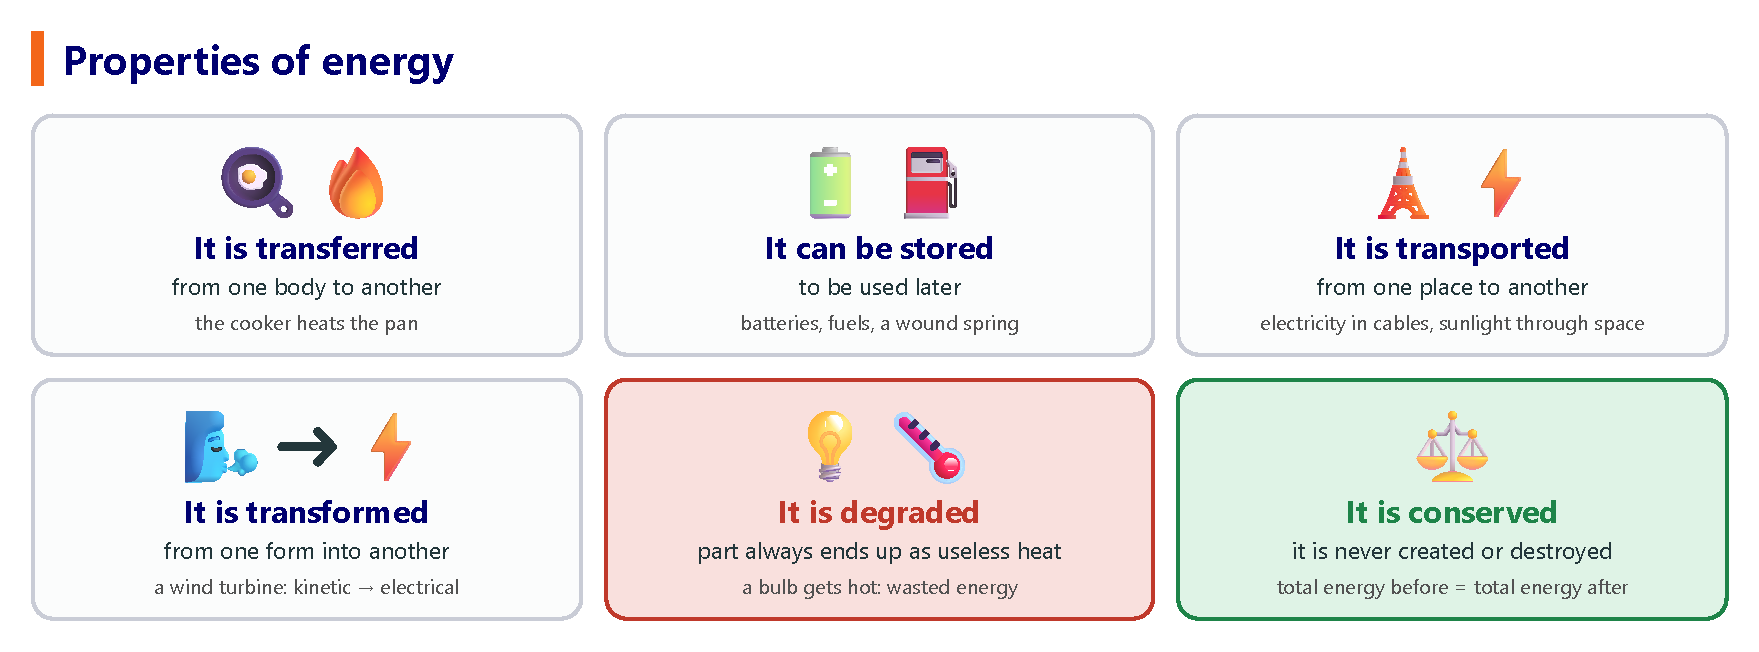
\includegraphics[width=\textwidth]{FigurasSVG/Unit_9_Energy/pdf/energy_properties.pdf}
    \caption{The six properties of energy.}
    \label{fig:u9_energy_properties}
\end{figure}

\begin{example}
    \textbf{Energy transformation chain in an electric torch (flashlight)}: chemical energy (battery) \(\to\) electrical energy \(\to\) radiant energy (light) \(+\) thermal energy (degraded, warms the torch). The total energy transformed is conserved, but only the radiant energy is useful.
\end{example}

\begin{figure}[H]
    \centering
    % [FIGURA ORIGINAL] \includegraphics[width=\textwidth]{Unit_9/torch_chain}
    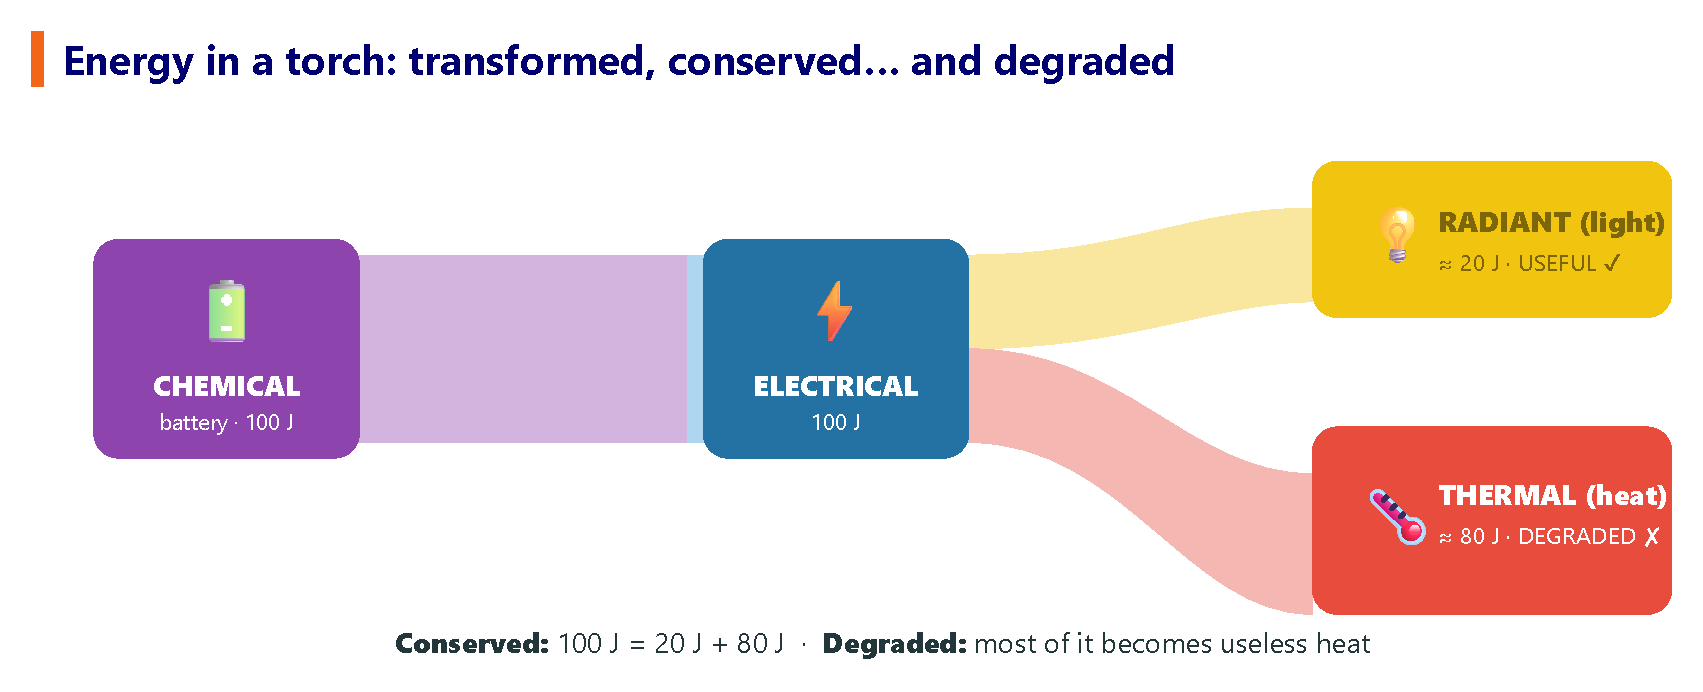
\includegraphics[width=\textwidth]{FigurasSVG/Unit_9_Energy/pdf/torch_chain.pdf}
    \caption{Energy in a torch: the total energy is conserved, but most of it is degraded into heat.}
    \label{fig:u9_torch_chain}
\end{figure}

\begin{exercise}
    For each device, write the chain of energy transformations from the energy source to the useful energy obtained: a) a wind turbine generating electricity; b) an electric kettle boiling water; c) a solar panel that heats water directly (no electricity involved).
    \begin{solu}
        \begin{enumerate}[label=\alph*)]
            \item Kinetic energy (wind) \(\to\) mechanical energy (rotating blades and generator) \(\to\) electrical energy.
            \item Electrical energy \(\to\) thermal energy (heats the water).
            \item Radiant energy (sunlight) \(\to\) thermal energy (heats the water directly).
        \end{enumerate}
    \end{solu}
\end{exercise}

\begin{exercise}
    A ball is dropped from a height and bounces several times, each time reaching a lower height than the previous one. Using the properties of energy, explain why this happens, and say whether any energy is destroyed.
    \begin{solu}
        At each bounce, part of the ball's mechanical energy is \textbf{transformed} into thermal energy and sound due to friction with the air and deformation on impact; this is energy \textbf{degradation}, so less useful (mechanical) energy is available for the next bounce, and it reaches a lower height each time. No energy is destroyed: the total energy is always \textbf{conserved}, it is just transformed into less useful forms.
    \end{solu}
\end{exercise}

\subsection{How bodies exchange energy}

\begin{itemize}
    \item \negsubro{In the form of heat}: bodies at different temperatures exchange energy until they reach the same temperature (e.g.\ ice melting absorbs heat from the air).
    \item \negsubro{In the form of mechanical work}: happens when a force causes a movement (e.g.\ pulling back a bow, pushing a shopping trolley).
\end{itemize}

\begin{figure}[H]
    \centering
    % [FIGURA ORIGINAL] \includegraphics[width=\textwidth]{Unit_9/heat_work}
    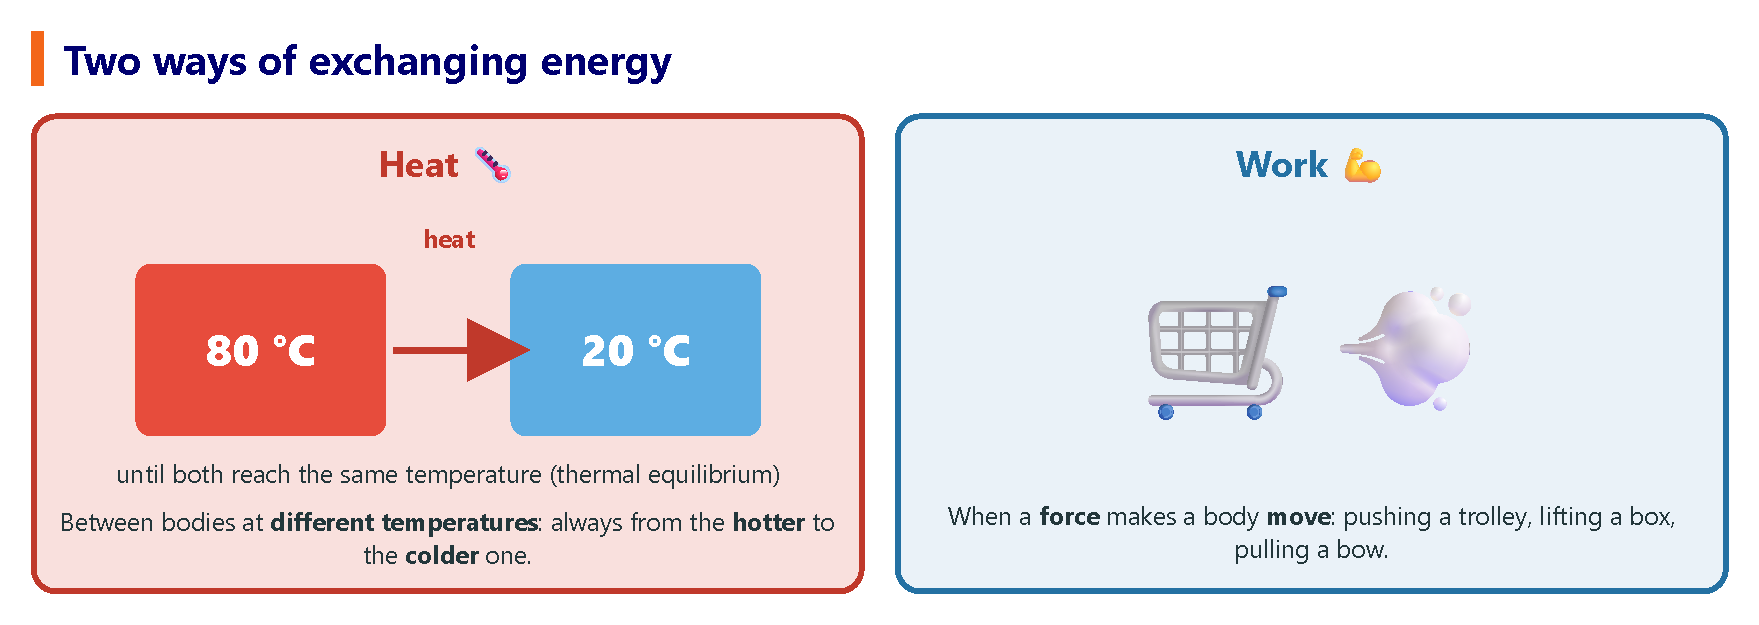
\includegraphics[width=\textwidth]{FigurasSVG/Unit_9_Energy/pdf/heat_work.pdf}
    \caption{Bodies exchange energy as heat or as work.}
    \label{fig:u9_heat_work}
\end{figure}

\begin{exercise}
    Identify the energy property involved in each situation: a) when we plug in a hairdryer, a current of air appears; b) a mobile phone battery lasts three days; c) when we put a bottle of water in the fridge, it cools down; d) light bulbs that heat up are not very efficient; e) high-voltage cables carry electricity across the country.
    \begin{solu}
        \begin{enumerate}[label=\alph*)]
            \item Energy is \textbf{transformed} (electrical into kinetic and thermal).
            \item Energy is \textbf{stored} (chemical energy in the battery).
            \item Energy is \textbf{transferred} in the form of heat (from the water to the cold air in the fridge).
            \item Energy is \textbf{degraded} (part of the electrical energy becomes heat instead of light).
            \item Energy is \textbf{transported}.
        \end{enumerate}
    \end{solu}
\end{exercise}

\begin{exercise}
    The efficiency of a machine is the relationship between the energy we want to obtain from it and the energy it consumes. Which property of energy always makes the efficiency of a machine lower than 100\,\%?
    \begin{solu}
        \textbf{Energy degradation}: every time energy is transformed, part of it is converted into non-useful heat, so a machine can never return 100\,\% of the energy it consumes as useful energy.
    \end{solu}
\end{exercise}

\begin{exercise}
    Two metal blocks, one at \qty{80}{\celsius} and the other at \qty{20}{\celsius}, are placed in contact inside an insulated box. Describe what happens to the energy of each block until they reach thermal equilibrium, and name the form in which the energy is exchanged.
    \begin{solu}
        Heat flows from the hotter block (\qty{80}{\celsius}) to the colder one (\qty{20}{\celsius}) until both reach the same intermediate temperature (thermal equilibrium). The energy is exchanged \textbf{in the form of heat}; no mechanical work is done, since neither block moves.
    \end{solu}
\end{exercise}

\subsection{Effects of heat on matter}

\begin{definition}[Specific heat capacity]
    The amount of heat needed to raise the temperature of \qty{1}{\kg} of a substance by \qty{1}{\celsius}. Its symbol is \(c\), and its SI unit is \unit{\joule\per\kg\per\celsius}.
    \begin{equation*}
        Q = m \cdot c \cdot \Delta T
    \end{equation*}
\end{definition}

Water has a very high specific heat, \(c_{\text{water}} = \qty{4180}{\joule\per\kg\per\celsius}\) (equivalent to \(\qty{1}{\calorie}/(\text{g} \cdot {}^{\circ}\text{C})\)): this is why water heats up and cools down more slowly than most other substances, and why places near the coast tend to have milder climates than places far from the sea.

\begin{figure}[H]
    \centering
    % [FIGURA ORIGINAL] \includegraphics[width=\textwidth]{Unit_9/specific_heat}
    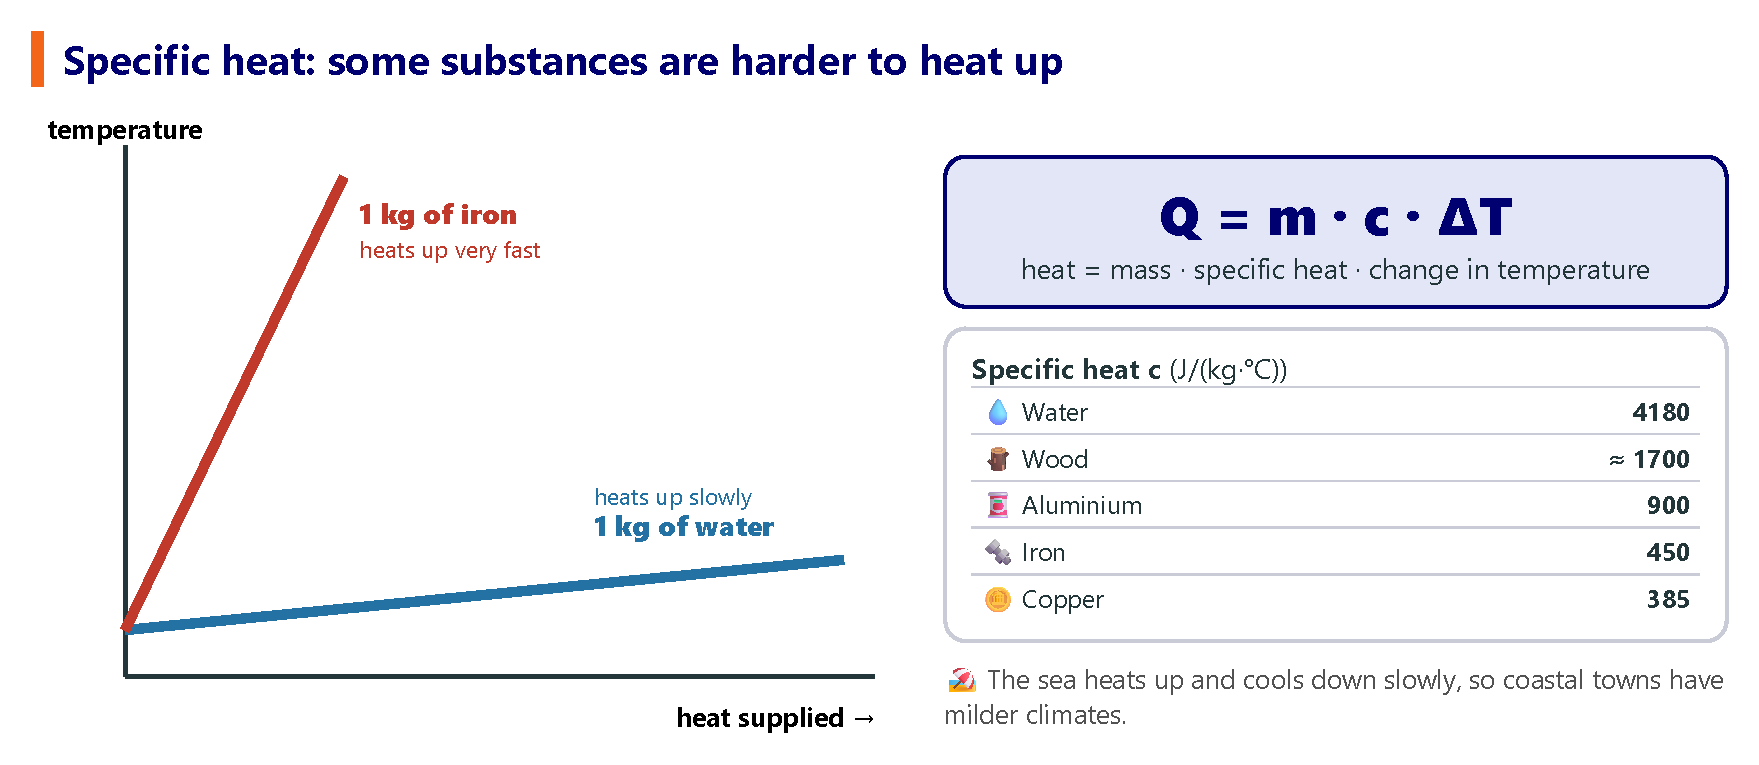
\includegraphics[width=\textwidth]{FigurasSVG/Unit_9_Energy/pdf/specific_heat.pdf}
    \caption{With the same heat, iron gets much hotter than water: water has a very high specific heat.}
    \label{fig:u9_specific_heat}
\end{figure}

\begin{example}
    \textbf{How much heat is needed to raise the temperature of \qty{2}{\kg} of water from \qty{18}{\celsius} to \qty{38}{\celsius}?}
    \begin{equation*}
        Q = m \cdot c \cdot \Delta T = \qty{2}{\kg} \cdot 4180 \dfrac{\text{J}}{\text{kg} \cdot {}^{\circ}\text{C}} \cdot (38 - 18)\ {}^{\circ}\text{C} = \textbf{167 200 J} \approx \textbf{167.2 kJ}
    \end{equation*}
\end{example}

\begin{exercise}
    Calculate the heat needed to raise the temperature of \qty{0.5}{\kg} of water from \qty{15}{\celsius} to \qty{100}{\celsius} in a kettle. Give the answer in kJ and in kcal.
    \begin{solu}
        \(Q = \qty{0.5}{\kg} \cdot 4180 \dfrac{\text{J}}{\text{kg} \cdot {}^{\circ}\text{C}} \cdot (100-15)\ {}^{\circ}\text{C} = \qty{177650}{\joule} \approx \qty{177.65}{\kilo\joule}\). \\
        In kcal: \(\qty{177650}{\joule} \cdot \dfrac{\qty{1}{\calorie}}{\qty{4.18}{\joule}} \approx \qty{42500}{\calorie} \approx \textbf{42.5 kcal}\).
    \end{solu}
\end{exercise}

\begin{exercise}
    A \qty{1.5}{\kg} block of an unknown metal absorbs \qty{13500}{\joule} of heat, and its temperature rises from \qty{20}{\celsius} to \qty{45}{\celsius}. Calculate its specific heat capacity.
    \begin{solu}
        From \(Q = m \cdot c \cdot \Delta T\): \(c = \dfrac{Q}{m \cdot \Delta T} = \dfrac{\qty{13500}{\joule}}{\qty{1.5}{\kg} \cdot (45-20)\ {}^{\circ}\text{C}} = \dfrac{13500}{37.5} = \textbf{360}\ \unit{\joule\per\kg\per\celsius}\).
    \end{solu}
\end{exercise}

\begin{impt}
    \negsubro{Thermal expansion}: most substances increase in volume when their temperature rises, and decrease in volume when it falls: they \textbf{expand} on heating and \textbf{contract} on cooling. Gases expand the most, followed by liquids, and then solids.
\end{impt}

\begin{figure}[H]
    \centering
    % [FIGURA ORIGINAL] \includegraphics[width=\textwidth]{Unit_9/thermal_expansion}
    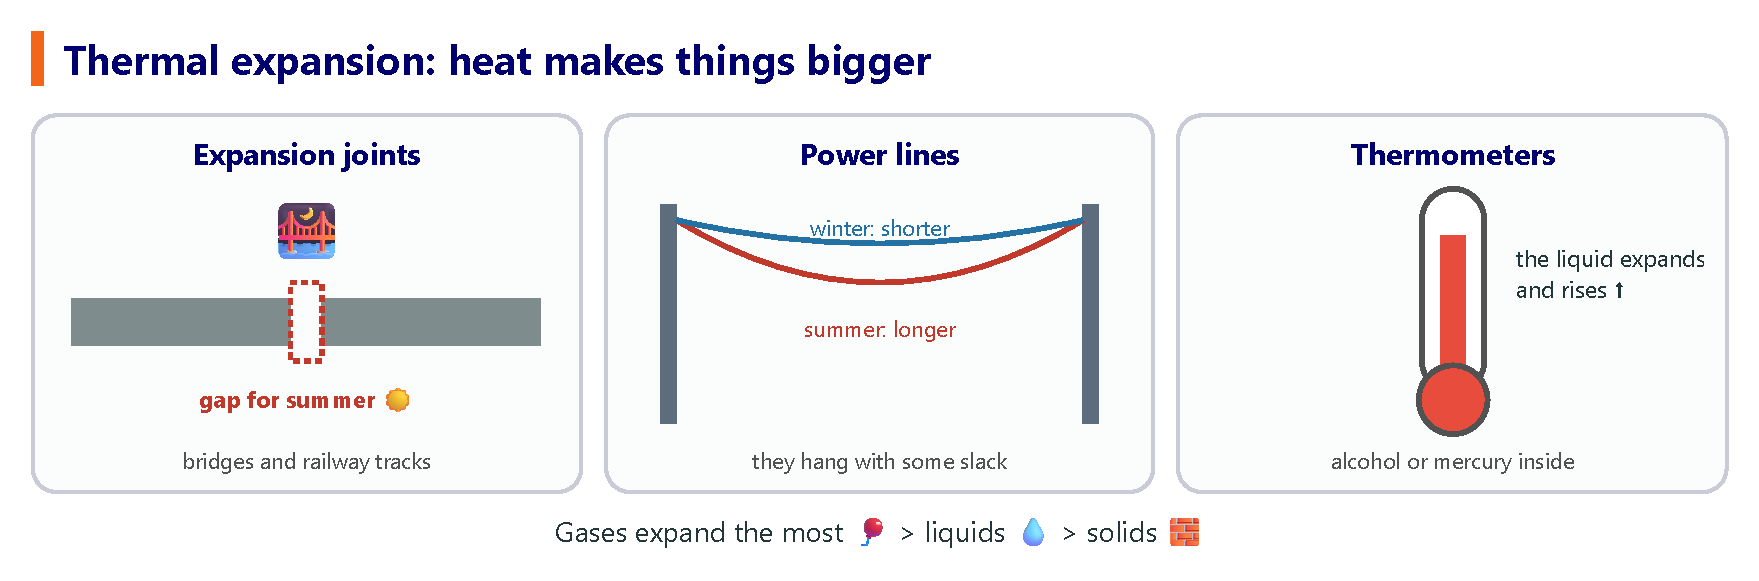
\includegraphics[width=\textwidth]{FigurasSVG/Unit_9_Energy/pdf/thermal_expansion.pdf}
    \caption{Everyday examples of thermal expansion.}
    \label{fig:u9_thermal_expansion}
\end{figure}

\begin{exercise}
    Explain why overhead electrical power lines are hung with some slack between the pylons, instead of being stretched tight.
    \begin{solu}
        In summer, the metal cables heat up and \textbf{expand}, becoming slightly longer; the slack allows this without the cables snapping or being damaged. In winter, the cables cool down and contract again.
    \end{solu}
\end{exercise}

\begin{exercise}
    State whether solids, liquids or gases expand the most when heated, and explain why a hot-air balloon rises when the air inside it is heated.
    \begin{solu}
        \textbf{Gases} expand the most, followed by liquids, and then solids. When the air inside the balloon is heated, it \textbf{expands} and becomes less dense than the cooler air outside; this makes the balloon (and the air inside it) buoyant, so it rises.
    \end{solu}
\end{exercise}

%----------------------------------------------------------------------------------------

\section{Energy sources}

\begin{definition}[Energy source]
    Any material or natural resource that can be used to obtain usable energy.
\end{definition}

\begin{figure}[H]
    \centering
    % [FIGURA ORIGINAL] \includegraphics[width=\textwidth]{Unit_9/sources}
    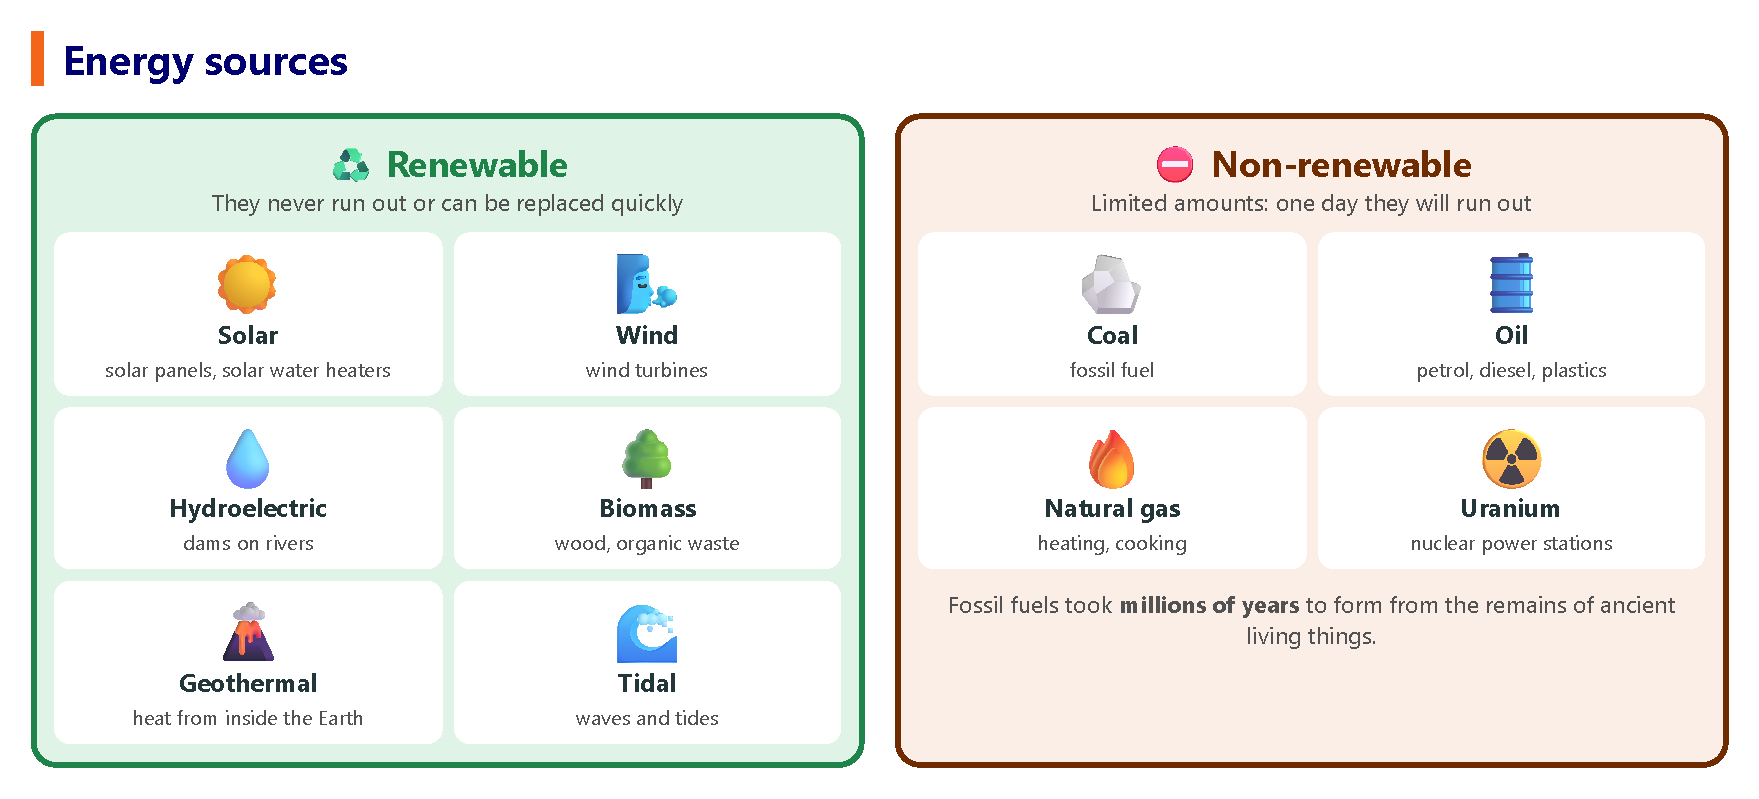
\includegraphics[width=\textwidth]{FigurasSVG/Unit_9_Energy/pdf/sources.pdf}
    \caption{Renewable and non-renewable energy sources.}
    \label{fig:u9_sources}
\end{figure}

\begin{impt}
    \negsubro{Direct use vs.\ electricity generation}: an energy source can be used \textbf{directly} (e.g.\ burning biomass for heating, sunlight heating water) or used to \textbf{generate electricity}, usually by rotating a turbine connected to a generator (in hydroelectric, wind, solar, thermal or nuclear power stations).
\end{impt}

\begin{exercise}
    Classify these energy sources as renewable or non-renewable, and say whether each is used \textbf{directly} or to \textbf{generate electricity}: a) natural gas burnt in a power station; b) firewood burnt in a fireplace; c) sunlight in solar panels that heat water directly; d) uranium in a nuclear power station.
    \begin{solu}
        \begin{enumerate}[label=\alph*)]
            \item Non-renewable; used to generate electricity.
            \item Renewable (biomass); used directly.
            \item Renewable; used directly (no electricity is generated).
            \item Non-renewable; used to generate electricity.
        \end{enumerate}
    \end{solu}
\end{exercise}

\subsection{Wind energy in Castilla-La Mancha}

Castilla-La Mancha is one of the Spanish regions with the largest number of wind farms, thanks to its flat terrain and strong, steady winds. A \negsubro{wind turbine} transforms the \textbf{kinetic energy} of the wind into \textbf{electrical energy}: the wind turns the blades, which rotate a shaft connected to a generator.

\begin{figure}[H]
    \centering
    % [FIGURA ORIGINAL] \includegraphics[width=\textwidth]{Unit_9/wind_turbine}
    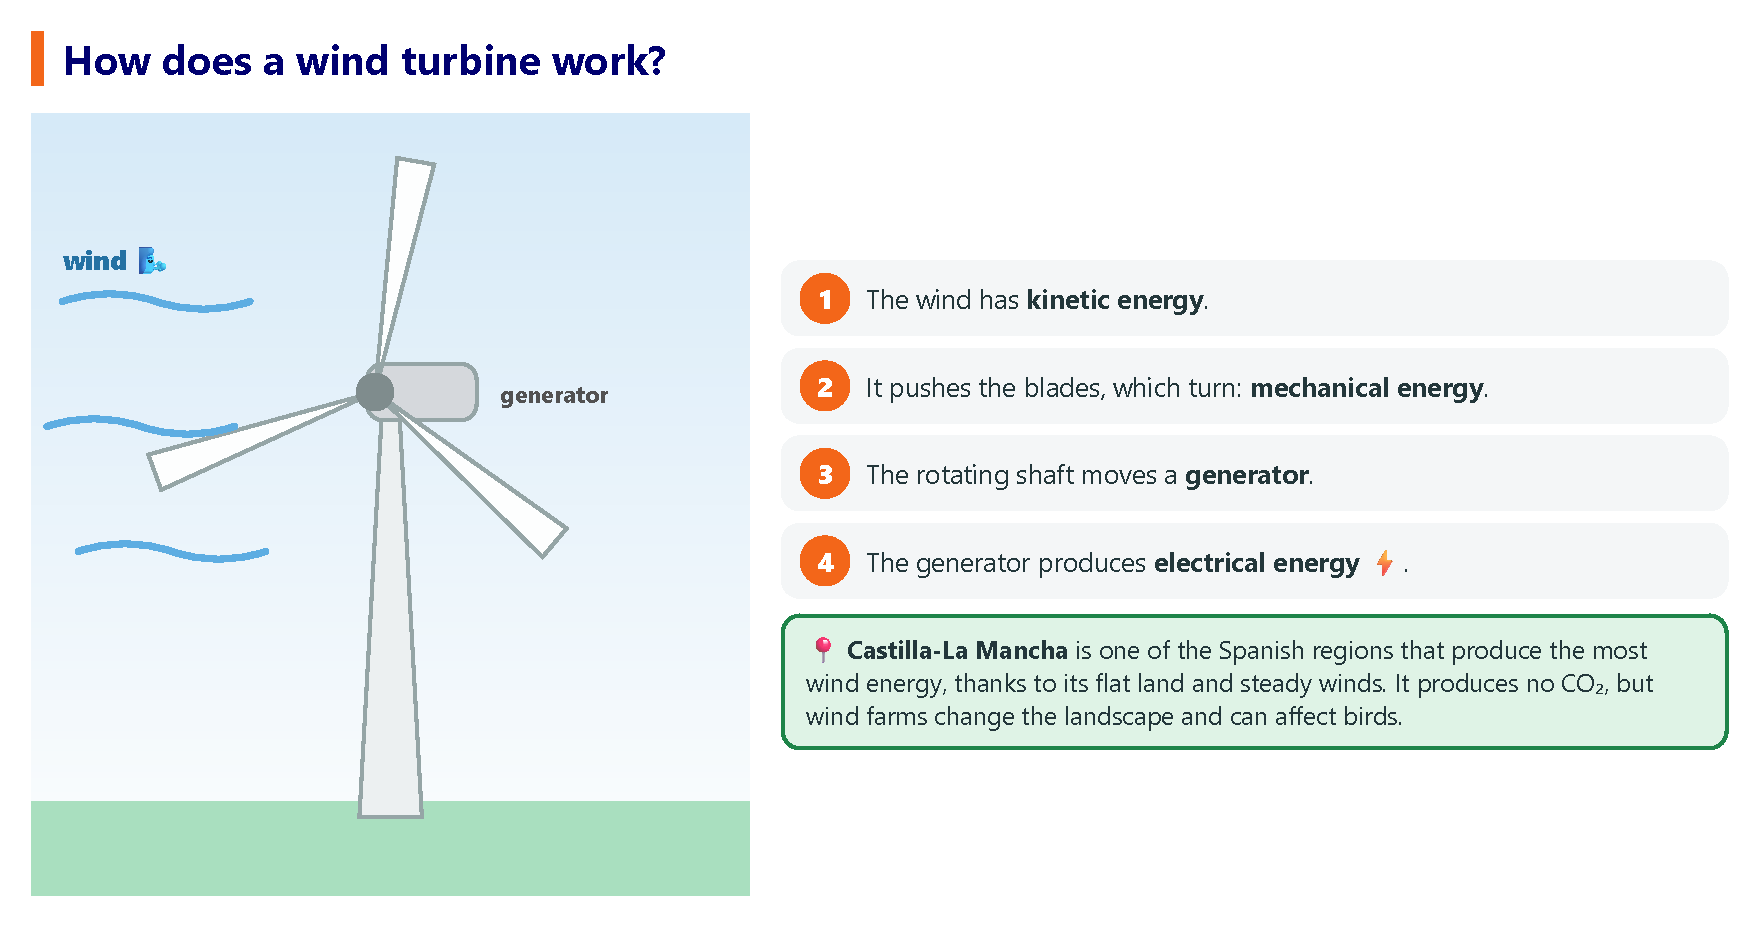
\includegraphics[width=\textwidth]{FigurasSVG/Unit_9_Energy/pdf/wind_turbine.pdf}
    \caption{How a wind turbine transforms the energy of the wind into electricity.}
    \label{fig:u9_wind_turbine}
\end{figure}

\begin{impt}
    \negsubro{Wind power in our region}: wind (eolic) energy is one of the main renewable sources produced in Castilla-La Mancha, together with solar energy, and the region is one of the leading wind-energy producers in Spain. This supplies a large share of the region's electricity without emitting greenhouse gases, but wind farms must be planned carefully, since they can affect birds, bats and the landscape.
\end{impt}

\begin{exercise}
    Explain two advantages and one disadvantage of installing wind farms in Castilla-La Mancha.
    \begin{solu}
        \textbf{Advantages} (any two): wind is a renewable, inexhaustible resource; generating electricity from wind does not emit \ch{CO2} or other pollutants; the region has strong, steady winds, making it an efficient location; it reduces dependence on imported fossil fuels. \\
        \textbf{Disadvantage} (any one): wind turbines change the landscape; they can affect birds and bats; electricity generation depends on the wind blowing, so it is not constant.
    \end{solu}
\end{exercise}

\begin{exercise}
    A wind turbine in Castilla-La Mancha has a rated power of \qty{2}{\mega\watt}. If it operates at full power for \qty{8}{\hour} in a day, calculate the energy it produces that day, in kWh and in MJ.
    \begin{solu}
        \(E = P \cdot t = \qty{2000}{\kilo\watt} \cdot \qty{8}{\hour} = \textbf{16000 kWh}\). \\
        In MJ: \(\qty{16000}{\kwh} \cdot \qty{3.6e6}{\joule\per\kwh} = \qty{5.76e10}{\joule} = \textbf{57600 MJ}\).
    \end{solu}
\end{exercise}

%\subsection{Electrical quantities}
%
%A generator produces an \textbf{electric current} (electric charges moving in an orderly way) inside an \textbf{electric circuit}.
%
%\begin{figure}[H]
%    \centering
%    \includegraphics[width=\textwidth]{Unit_9/circuit}
%    \caption{A simple electric circuit and the three electrical quantities.}
%    \label{fig:u9_circuit}
%\end{figure}
%
%\begin{exercise}
%    Name the basic parts of a simple electric circuit (battery, bulb) and explain the function of each one.
%    \begin{solu}
%        \textbf{Generator} (e.g.\ battery): produces the electric current. \\
%        \textbf{Wires/connectors}: made of a conductive material (e.g.\ copper); transport the current between components. \\
%        \textbf{Switch}: a control element that opens or closes the circuit, stopping or starting the current. \\
%        \textbf{Receiver} (e.g.\ bulb, motor): transforms the electric current into another form of energy (light, movement, etc.).
%    \end{solu}
%\end{exercise}
%
%
%\begin{exercise}
%    A charge of \qty{15}{\coulomb} flows through a wire in \qty{5}{\second}. Calculate the current intensity.
%    \begin{solu}
%        \(I = \dfrac{Q}{t} = \dfrac{\qty{15}{\coulomb}}{\qty{5}{\s}} = \textbf{3 A}\).
%    \end{solu}
%\end{exercise}
%
%\begin{exercise}
%    State which electrical quantity (current intensity, potential difference or resistance) is being described in each case: a) it is measured in volts; b) it opposes the flow of electric current; c) it is measured using an ammeter.
%    \begin{solu}
%        \begin{enumerate}[label=\alph*)]
%            \item Potential difference.
%            \item Resistance.
%            \item Current intensity.
%        \end{enumerate}
%    \end{solu}
%\end{exercise}

%\subsection{Ohm's law}
%
%\begin{impt}
%    \negsubro{Ohm's law} relates the three electrical quantities of a circuit:
%    \begin{equation*}
%        I = \dfrac{\Delta V}{R}
%    \end{equation*}
%    The current intensity through a conductor is directly proportional to the potential difference applied to it, and inversely proportional to its resistance.
%\end{impt}
%
%\begin{figure}[H]
%    \centering
%    \includegraphics[width=\textwidth]{Unit_9/ohm_law}
%    \caption{Ohm's law: the triangle helps us to isolate each quantity.}
%    \label{fig:u9_ohm_law}
%\end{figure}
%
%\begin{example}
%    \textbf{A bulb of resistance \qty{60}{\ohm} is connected to a \qty{12}{\volt} battery. What current flows through it?}
%    \begin{equation*}
%        I = \dfrac{\Delta V}{R} = \dfrac{\qty{12}{\volt}}{\qty{60}{\ohm}} = \textbf{0.2 A}
%    \end{equation*}
%\end{example}
%
%\begin{exercise}
%    A hairdryer connected to the \qty{230}{\volt} mains has a resistance of \qty{46}{\ohm}. Calculate the current intensity that flows through it.
%    \begin{solu}
%        \(I = \dfrac{\Delta V}{R} = \dfrac{\qty{230}{\volt}}{\qty{46}{\ohm}} = \textbf{5 A}\).
%    \end{solu}
%\end{exercise}
%
%\begin{exercise}
%    A current of \qty{0.5}{\ampere} flows through a resistor connected to a \qty{9}{\volt} battery. Calculate the resistance of the resistor.
%    \begin{solu}
%        From Ohm's law, \(R = \dfrac{\Delta V}{I} = \dfrac{\qty{9}{\volt}}{\qty{0.5}{\ampere}} = \textbf{18}\ \Omega\).
%    \end{solu}
%\end{exercise}
%
%\begin{exercise}
%    A resistor has a resistance of \qty{25}{\ohm}. What potential difference must be applied to it so that a current of \qty{2}{\ampere} flows through it?
%    \begin{solu}
%        From Ohm's law, \(\Delta V = I \cdot R = \qty{2}{\ampere} \cdot \qty{25}{\ohm} = \textbf{50 V}\).
%    \end{solu}
%\end{exercise}

%\subsection{Series and parallel circuits}
%
%\begin{figure}[H]
%    \centering
%    \includegraphics[width=\textwidth]{Unit_9/series_parallel}
%    \caption{Bulbs connected in series and in parallel.}
%    \label{fig:u9_series_parallel}
%\end{figure}
%
%\begin{example}
%    A string of old-style Christmas lights wired \textbf{in series} switches off completely if a single bulb breaks. Household electrical installations are wired \textbf{in parallel}: switching off one lamp, or a bulb breaking, does not switch off the other appliances connected to the mains.
%\end{example}
%
%
%\begin{exercise}
%    Say whether the bulbs in each situation are connected in series or in parallel, and justify your answer: a) when one bulb is unscrewed, all the other bulbs go off too; b) a fridge keeps working even if a lamp in another room is switched off.
%    \begin{solu}
%        \begin{enumerate}[label=\alph*)]
%            \item \textbf{Series}: there is a single path for the current, so removing one bulb interrupts the whole circuit.
%            \item \textbf{Parallel}: each appliance is on its own branch, so it works independently of the others.
%        \end{enumerate}
%    \end{solu}
%\end{exercise}
%
%\begin{exercise}
%    Three identical bulbs are connected \textbf{in series} to a \qty{12}{\volt} battery. If one bulb burns out, what happens to the other two? Explain.
%    \begin{solu}
%        In a series circuit there is only \textbf{one path} for the current. If one bulb burns out, it interrupts that path, so no current can flow anywhere in the circuit: the \textbf{other two bulbs also go off}.
%    \end{solu}
%\end{exercise}
%
%\begin{exercise}
%    Two lamps with different resistances are connected \textbf{in parallel} to the \qty{230}{\volt} mains supply. Explain why both lamps are subject to the same potential difference, and what this means for their brightness.
%    \begin{solu}
%        In a parallel circuit, every branch connects the same two points, so the potential difference across each branch equals the source voltage: both lamps have \qty{230}{\volt} across them. However, by Ohm's law (\(I = \Delta V / R\)), the lamp with the \textbf{lower resistance} draws a \textbf{higher current}, so it will shine \textbf{brighter}, even though both receive the same potential difference.
%    \end{solu}
%\end{exercise}

%----------------------------------------------------------------------------------------

\section{The environmental impact of energy}

Obtaining, transporting and using energy has consequences for the environment: resources are depleted, toxic waste is produced, and air, water and soil are polluted.

\begin{itemize}
    \item \negsubro{Acid rain}: when fossil fuels are burnt, the substances released combine with rainwater; this rain damages plants and can affect areas far from where the pollution was produced.
    \item \negsubro{Global warming}: burning fossil fuels increases the carbon dioxide in the atmosphere, which increases the natural greenhouse effect and raises the planet's average temperature.
\end{itemize}

\begin{table}[H]
    \centering
    \begin{tabular}{p{5.3cm}p{5.3cm}}
        \toprule
        \textbf{Renewable sources} & \textbf{Non-renewable sources} \\
        \midrule
        Do not emit harmful substances, but they can greatly change the landscape and the habitats of living things (e.g.\ wind turbines, large solar or hydroelectric power plants). &
        Fossil fuels emit \ch{CO2} and other greenhouse gases, and cause acid rain; extraction changes the land, and accidental spills cause pollution. Radioactive materials produce dangerous waste that must be stored securely. \\
        \bottomrule
    \end{tabular}
    \caption{Environmental impact of renewable and non-renewable energy sources.}
    \label{tab:u9_impact}
\end{table}

\begin{exercise}
    Match each cause with its environmental consequence: a) burning fossil fuels for transport; b) an oil tanker accident; c) a nuclear power station's radioactive waste. \newline
    Consequences: 1. large oil spills; 2. air pollution / global warming; 3. long-term, dangerous waste storage needs.
    \begin{solu}
        a) \(\to\) 2; \quad b) \(\to\) 1; \quad c) \(\to\) 3.
    \end{solu}
\end{exercise}

\begin{exercise}
    Explain how burning fossil fuels contributes to two different environmental problems studied in this unit.
    \begin{solu}
        Burning fossil fuels releases \ch{CO2}, which increases the natural \textbf{greenhouse effect} and causes \textbf{global warming}. It also releases sulfur and nitrogen oxides, which combine with water in the atmosphere and fall as \textbf{acid rain}, damaging plants and ecosystems, sometimes far from where the pollution was originally produced.
    \end{solu}
\end{exercise}

%----------------------------------------------------------------------------------------

\section{The energy we use}

\begin{itemize}
    \item \negsubro{Primary energy}: energy obtained directly from a source in nature (e.g.\ the chemical energy in coal, or the kinetic energy of wind), used directly or transformed.
    \item \negsubro{Final energy}: the energy that is actually supplied to and used by the consumer (e.g.\ electricity, petrol), after it has been transformed and transported.
\end{itemize}

\begin{impt}
    A country that consumes more energy than it produces is an \negsubro{energy importer}; a country that produces more than it consumes is an \negsubro{energy exporter}.
\end{impt}

Figure~\ref{fig:u9_energy_mix} shows the world energy mix by primary source in 2021, used in the exercise below.

\begin{figure}[H]
    \centering
    % [FIGURA ORIGINAL] \includegraphics[width=0.95\textwidth]{Unit_9/energy_mix}
    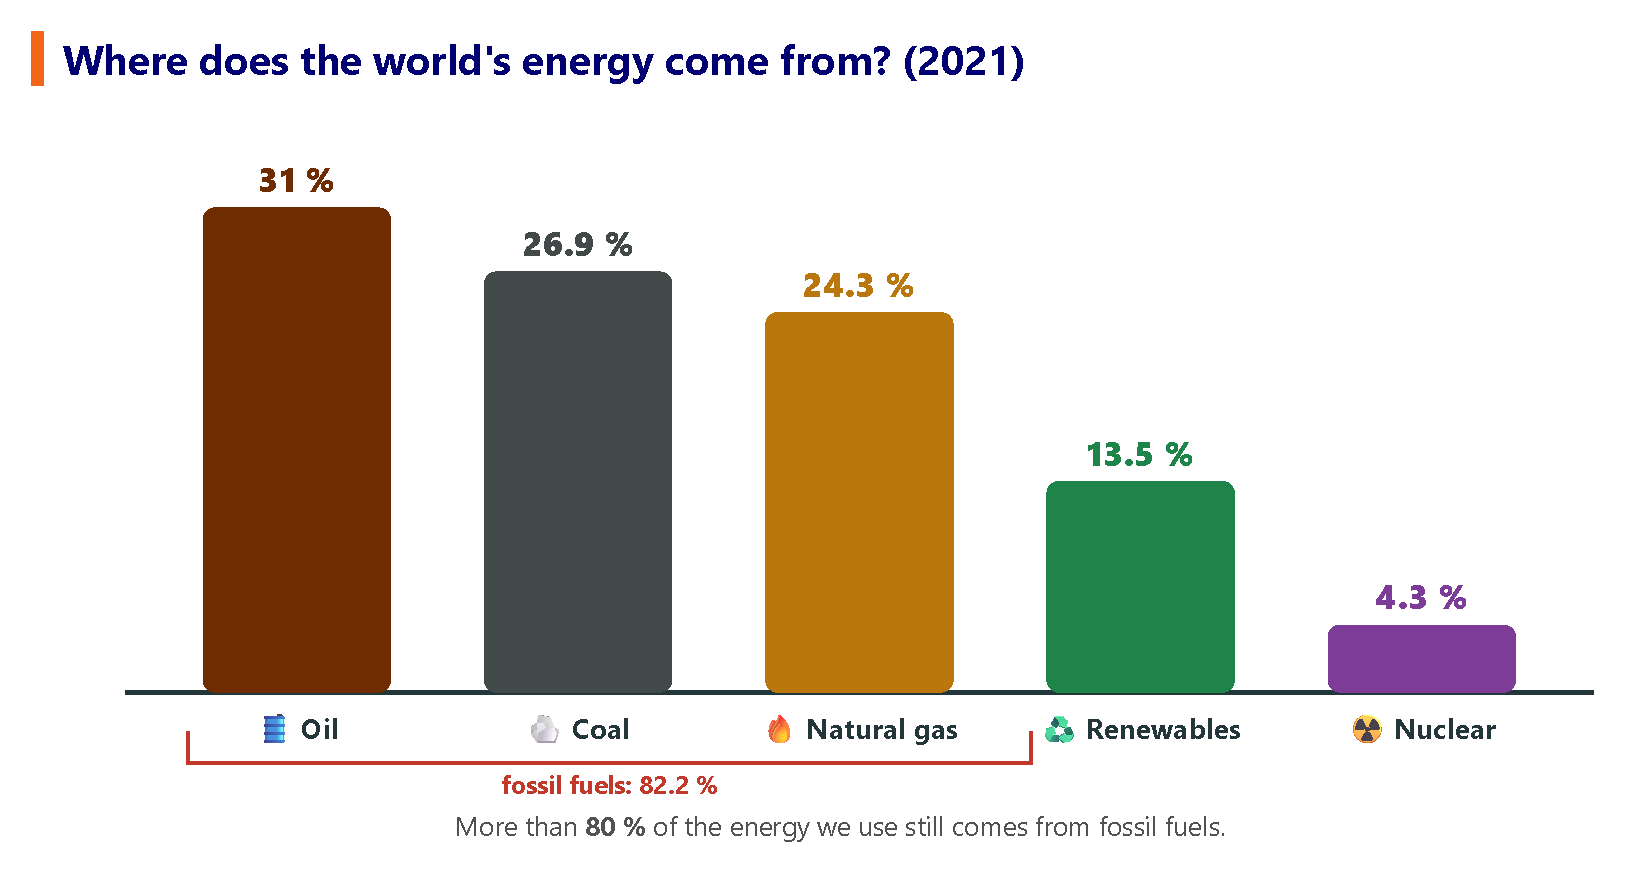
\includegraphics[width=0.95\textwidth]{FigurasSVG/Unit_9_Energy/pdf/energy_mix.pdf}
    \caption{World primary energy consumption by source, 2021.}
    \label{fig:u9_energy_mix}
\end{figure}

\begin{exercise}
    Worldwide in 2021, total energy consumption by primary source was distributed as follows: petroleum 31\,\%, natural gas 24.3\,\%, coal 26.9\,\%, nuclear 4.3\,\%, renewables 13.5\,\%, out of a total of \num{14220} Mtoe (million tonnes of oil equivalent). Calculate the amount of energy, in Mtoe, consumed from petroleum and from renewables.
    \begin{solu}
        Petroleum: \(14220 \cdot \dfrac{31}{100} \approx 4408.2\) Mtoe. \\
        Renewables: \(14220 \cdot \dfrac{13.5}{100} \approx 1919.7\) Mtoe.
    \end{solu}
\end{exercise}

\begin{exercise}
    Explain why electrical energy appears in the \textbf{final} energy consumption of a country, but not directly in its \textbf{primary} energy consumption.
    \begin{solu}
        Electricity is not a primary energy source itself; it is generated by transforming primary sources (fossil fuels, nuclear, wind, water, sun, etc.). Once generated, it is counted as a form of \textbf{final} energy, since it is what is actually delivered to and used by the consumer.
    \end{solu}
\end{exercise}

\begin{exercise}
    A country produced 145 Mtoe of primary energy in a given year but consumed 165 Mtoe. Was that country an energy importer or an energy exporter that year? Justify your answer and calculate the energy deficit, in Mtoe.
    \begin{solu}
        Since consumption (165 Mtoe) is greater than production (145 Mtoe), the country was an \textbf{energy importer} that year: it needed to bring in energy from abroad to cover its needs. \\
        Deficit \(= 165 - 145 = \textbf{20 Mtoe}\).
    \end{solu}
\end{exercise}

%----------------------------------------------------------------------------------------

\section{Energy saving and sustainable development}

\begin{definition}[Sustainable development]
    Development that meets present energy needs without wasting resources or causing unnecessary environmental damage, so that future generations can also meet their needs.
\end{definition}

\begin{itemize}
    \item \negsubro{Design of efficient products and buildings}: energy-efficient vehicles and appliances; well-insulated houses to prevent energy losses.
    \item \negsubro{Local energy sources}: installing solar panels; using the natural course of rivers; using local organic waste as biomass.
    \item \negsubro{Avoiding unnecessary consumption}: using public transport; buying only what is needed; consuming local products.
    \item \negsubro{At home}: use energy-saving light bulbs; switch off lights and devices when not in use; use heating and air conditioning sensibly; do not waste hot water.
\end{itemize}

\begin{figure}[H]
    \centering
    % [FIGURA ORIGINAL] \includegraphics[width=\textwidth]{Unit_9/energy_saving}
    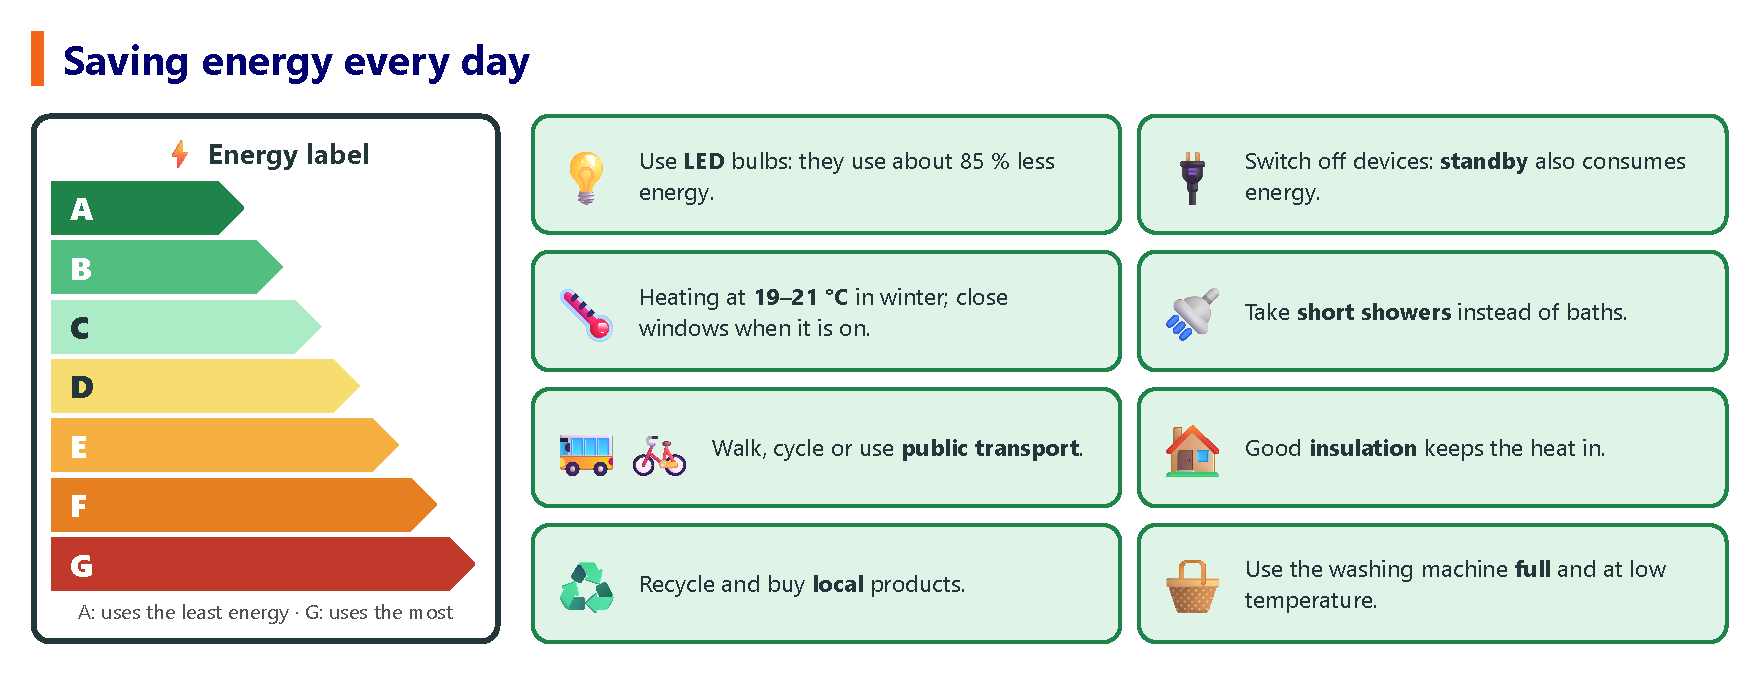
\includegraphics[width=\textwidth]{FigurasSVG/Unit_9_Energy/pdf/energy_saving.pdf}
    \caption{The energy label and some simple ways to save energy.}
    \label{fig:u9_energy_saving}
\end{figure}

\begin{exercise}
    A category D fridge (average consumption) uses \qty{600}{\kwh} per year. Category A fridges consume about 55\,\% \textbf{less} than average, and category G fridges consume about 125\,\% \textbf{more} than average.
    \begin{enumerate}[label=\letraminuscula]
        \item How much would a category A fridge consume per year?
        \item How much would a category G fridge consume per year?
    \end{enumerate}
    \begin{solu}
        \begin{enumerate}[label=\alph*)]
            \item \(\qty{600}{\kwh} \cdot (1 - 0.55) = 600 \cdot 0.45 = \qty{270}{\kwh}\) per year.
            \item \(\qty{600}{\kwh} \cdot (1 + 1.25) = 600 \cdot 2.25 = \qty{1350}{\kwh}\) per year.
        \end{enumerate}
    \end{solu}
\end{exercise}

\begin{exercise}
    Decide whether each action saves energy, and explain why: a) unplugging electrical devices that are not in use; b) opening windows in winter for ventilation while the heating is on; c) using energy-saving light bulbs.
    \begin{solu}
        \begin{enumerate}[label=\alph*)]
            \item \textbf{Saves energy}: many devices keep consuming small amounts of electricity on standby.
            \item \textbf{Does not save energy} (if done with the heating on): heat escapes and the heating has to work harder to compensate. (Brief ventilation with the heating \textit{off} is fine.)
            \item \textbf{Saves energy}: LED/energy-saving bulbs turn a higher percentage of the electrical energy into light and less into wasted heat, i.e.\ they degrade less energy.
        \end{enumerate}
    \end{solu}
\end{exercise}

\begin{exercise}
    A family replaces 10 incandescent light bulbs (\qty{60}{\watt} each) with 10 LED bulbs (\qty{9}{\watt} each), used for an average of \qty{4}{\hour} per day. Calculate the energy saved per day, in kWh.
    \begin{solu}
        Incandescent bulbs: \(10 \cdot \qty{60}{\watt} = \qty{600}{\watt} = \qty{0.6}{\kilo\watt}\); \(\qty{0.6}{\kilo\watt} \cdot \qty{4}{\hour} = \qty{2.4}{\kwh}\). \\
        LED bulbs: \(10 \cdot \qty{9}{\watt} = \qty{90}{\watt} = \qty{0.09}{\kilo\watt}\); \(\qty{0.09}{\kilo\watt} \cdot \qty{4}{\hour} = \qty{0.36}{\kwh}\). \\
        Energy saved \(= 2.4 - 0.36 = \textbf{2.04 kWh per day}\).
    \end{solu}
\end{exercise}

%----------------------------------------------------------------------------------------

\section*{Summary}

\begin{itemize}
    \item \textbf{Energy}: the capacity of a body to produce changes; measured in joules (also kJ, cal, kWh, toe).
    \item \textbf{Forms of energy}: kinetic, potential (gravitational and elastic), mechanical, thermal, electrical, radiant, chemical and nuclear.
    \item \textbf{Properties}: energy can be transferred, stored, transported and transformed; it is always conserved (as a total) but part of it is degraded (turned into unusable heat) every time it is transformed.
    \item \textbf{Effects of heat}: specific heat \(c\) measures the heat needed to raise \qty{1}{\kg} of a substance by \qty{1}{\celsius} (\(Q = mc\Delta T\)); most substances expand when heated and contract when cooled (thermal expansion).
    \item \textbf{Energy sources}: renewable (wind, water, sun, biomass, geothermal) do not run out; non-renewable (fossil fuels, radioactive materials) are limited and eventually run out. Wind energy is one of the main renewable sources produced in Castilla-La Mancha.
%    \item \textbf{Electrical quantities}: current intensity \(I\) (A), potential difference \(\Delta V\) (V) and resistance \(R\) (\(\Omega\)), related by \textbf{Ohm's law}, \(I = \Delta V / R\). Circuits can be wired in \textbf{series} (single path) or in \textbf{parallel} (independent branches).
    \item \textbf{Environmental impact}: burning fossil fuels causes acid rain and global warming; all energy sources have some impact on the landscape or habitats.
    \item \textbf{Primary vs.\ final energy}: primary energy comes directly from a source; final energy is what is actually delivered to and used by the consumer (e.g.\ electricity).
    \item \textbf{Sustainable development}: saving energy and using efficient, local and renewable resources to meet our needs without compromising future generations.
\end{itemize}

\section{Vocabulary}

\begin{vocabulary}[Energy]
    A physical quantity that measures the capacity of a body to produce changes in itself or in other bodies. \newline
    \textbf{Translation to Spanish}: Energía
\end{vocabulary}

\begin{vocabulary}[Kinetic energy]
    Energy a body has because it is moving. \newline
    \textbf{Translation to Spanish}: Energía cinética
\end{vocabulary}

\begin{vocabulary}[Potential energy]
    Energy a body has because of its position or state (e.g.\ its height, or being stretched). \newline
    \textbf{Translation to Spanish}: Energía potencial
\end{vocabulary}

\begin{vocabulary}[Energy source]
    Any material or natural resource that can be used to obtain usable energy. \newline
    \textbf{Translation to Spanish}: Fuente de energía
\end{vocabulary}

\begin{vocabulary}[Renewable]
    An energy source whose resources can be replaced after use, or that never run out. \newline
    \textbf{Translation to Spanish}: Renovable
\end{vocabulary}

\begin{vocabulary}[Non-renewable]
    An energy source whose resources are limited and cannot be replaced once consumed. \newline
    \textbf{Translation to Spanish}: No renovable
\end{vocabulary}

\begin{vocabulary}[Electric current]
    Electric charges moving in an orderly way through a conductor. \newline
    \textbf{Translation to Spanish}: Corriente eléctrica
\end{vocabulary}

\begin{vocabulary}[Specific heat capacity]
    The amount of heat needed to raise the temperature of \qty{1}{\kg} of a substance by \qty{1}{\celsius}. \newline
    \textbf{Translation to Spanish}: Calor específico
\end{vocabulary}

\begin{vocabulary}[Thermal expansion]
    The increase in volume of a substance when its temperature rises. \newline
    \textbf{Translation to Spanish}: Dilatación térmica
\end{vocabulary}

\begin{vocabulary}[Wind energy]
    Kinetic energy of the wind, used directly or transformed into electrical energy by wind turbines. \newline
    \textbf{Translation to Spanish}: Energía eólica
\end{vocabulary}

\begin{vocabulary}[Ohm's law]
    The relationship between current intensity, potential difference and resistance in a circuit: \(I = \Delta V / R\). \newline
    \textbf{Translation to Spanish}: Ley de Ohm
\end{vocabulary}

\begin{vocabulary}[Series circuit]
    A circuit in which components are connected one after another along a single path. \newline
    \textbf{Translation to Spanish}: Circuito en serie
\end{vocabulary}

\begin{vocabulary}[Parallel circuit]
    A circuit in which components are connected on separate branches between the same two points. \newline
    \textbf{Translation to Spanish}: Circuito en paralelo
\end{vocabulary}

\begin{vocabulary}[Energy degradation]
    The loss, during any energy transformation, of part of the energy as unusable heat. \newline
    \textbf{Translation to Spanish}: Degradación de la energía
\end{vocabulary}

\begin{vocabulary}[Primary energy]
    Energy obtained directly from a natural source. \newline
    \textbf{Translation to Spanish}: Energía primaria
\end{vocabulary}

\begin{vocabulary}[Final energy]
    The energy actually supplied to and used by the consumer. \newline
    \textbf{Translation to Spanish}: Energía final
\end{vocabulary}

\begin{vocabulary}[Sustainable development]
    Development that meets present needs without compromising the ability of future generations to meet theirs. \newline
    \textbf{Translation to Spanish}: Desarrollo sostenible
\end{vocabulary}
